\documentclass[12pt]{article}
\pagestyle{empty}
\usepackage{amsmath, amssymb, amsthm}
\usepackage{latexsym, epsfig, ulem, cancel, multicol, hyperref}
\usepackage{graphicx, tikz, subfigure,pgfplots}
\usepackage[margin=1in]{geometry}
\setlength{\parindent}{0pt}
\usepackage{multirow}
\usepackage{mathtools}
\usepackage{verbatim}
\usepackage{tikz}
\usepackage{pgfplots}
\setlength{\parskip}{1ex}

\newcommand{\T}[0]{\top}
\newcommand{\F}[0]{\bot}
\newcommand{\liminfty}[1]{\lim_{#1 \to \infty}}
\newcommand{\limzero}[1]{\lim_{#1 \to 0}}
\newcommand{\limto}[1]{\lim_{#1}}
\newcommand{\Z}{\mathbb{Z}}
\newcommand{\R}{\mathbb{R}}
\newcommand{\C}{\mathbb{C}}
\newcommand{\Q}{\mathbb{Q}}
\newcommand{\odd}[0]{\mathbb{Z} - 2\mathbb{Z}}
\newcommand{\lineint}[1]{\int_{#1}}
\newcommand{\pypx}[2]{\frac{\partial #1}{\partial #2}}
\newcommand{\divg}{\nabla \cdot}
\newcommand{\curl}{\nabla \times}
\newcommand{\dydx}[2]{\frac{d #1}{d #2}}
\newcommand{\sqbkt}[1]{\left[ #1 \right]}
\newcommand{\paren}[1]{\left( #1 \right)}
\newcommand{\tribkt}[1]{\left< #1 \right>}
\newcommand{\abso}[1]{\left|#1 \right|}
\newcommand{\zero}{\{0\}}
\newcommand{\then}{\rightarrow}
\newcommand{\nonneg}{\Z^+ \cup \{0\}}
\DeclarePairedDelimiter\ceil{\lceil}{\rceil}
\DeclarePairedDelimiter\floor{\lfloor}{\rfloor}
\newcommand{\union}[2]{\bigcup_{#1}^{#2}}
\newcommand{\inter}[2]{\bigcap_{#1}^{#2}}
\newcommand{\openclose}[1]{\left( #1 \right]}
\newcommand{\closeopen}[1]{\left[ #1 \right)}
\newcommand{\compo}[2]{#1 e^{i #2}}
\newcommand{\laplase}{\bigtriangleup}
\newcommand{\bra}[1]{\left< #1 \right|}
\newcommand{\ket}[1]{\left| #1 \right>}
\newcommand{\braket}[2]{\left< #1 \mid #2 \right>}
\newcommand{\ketbra}[2]{\left| #1 \right> \left< #2 \right|}
\newcommand{\ketpsit}{\ket{\psi(t)}}
\newcommand{\ketphit}{\ket{\phi(t)}}
\newcommand{\ham}{\mathbf{H}}
\newcommand{\unx}{\hat{\mathbf{x}}}
\newcommand{\uny}{\hat{\mathbf{y}}}
\newcommand{\unz}{\hat{\mathbf{z}}}
\newcommand{\uni}{\hat{\mathbf{i}}}
\newcommand{\unj}{\hat{\mathbf{j}}}
\newcommand{\unk}{\hat{\mathbf{k}}}
\newcommand{\uns}{\hat{\mathbf{s}}}
\newcommand{\unr}{\hat{\mathbf{r}}}
\newcommand{\untheta}{\hat{\boldsymbol\theta}}
\newcommand{\unphi}{\hat{\boldsymbol\phi}}
\newcommand{\unrho}{\hat{\boldsymbol\rho}}


\newcommand{\wsnumber}{1}
\newcommand{\wstopic}{Vectors}
\pgfplotsset{
    every linear axis/.append style={
       axis x line=center,
       axis y line=center,
       xlabel={$x$},
       ylabel={$y$}
    },
    every axis plot/.append style={thick,mark=none}
}
\tikzset{
    point/.style={circle,draw,fill,minimum width=0.3ex,inner sep=0pt,outer sep=0pt},
    every label/.append style={black}
}


\usepackage[margin=1in]{geometry}
\usepackage{amsmath, amssymb, amsthm, graphicx, hyperref}
\usepackage{enumerate}
\usepackage{fancyhdr}
\usepackage{multirow, multicol}
\usepackage{tikz}
\pagestyle{fancy}
\fancyhead[RO]{Dennis Li}
\fancyhead[LO]{Analytical Mechanics }
\usepackage{comment}
\newif\ifshow
\showfalse

\ifshow
  \newenvironment{solution}{\textbf{Solution.}}{}
\else
  \excludecomment{solution}
\fi

\renewcommand{\thefootnote}{\fnsymbol{footnote}}
\usepackage{comment}


\newtheorem*{remark}{Remark}


\begin{document}
\begin{center}
\ifshow
  \textbf{\Large Problem Set 01 Solution}\\
\else
  \textbf{\Large Problem Set 01}\\
\fi
Instructor \\ Prof. Gabe\\
\end{center}

\hrule

\vspace{0.2cm}

\section{Which statement is frame dependent?}

\begin{enumerate}
    \item A is at rest.

    This is true in $A's$ own reference frame, or a reference frame in which $A$ is at rest. This is not true for all frame, and not true for some inertial frame that is moving at constant velocity with respect to $A$.

    \item $A$ is currently 5 meters away from $B$

    This is true for all frame, and is true for all inertial frame since we are discussing non-relativistic. 

    \item $A$ is moving at 6 $m/s$.

    This is not true in all frame, and not true in all reference fame. Example being the frame $A$ where $A$ is at rest. 

    \item $A$ is moving 6 $m/s$ faster than $B$.

    This is not true for all frame, since in a frame relatively at rest with respect to $A$, $B$ is the only particle moving and $A$ is at rest. And it is not true for all inertial frame since a frame defined just now was inertial. 

    \item $A$ is at the same place as it was 5$s$ ago. 

    This is not true for frames that are moving relative to $A$. It cannot be true for all frame and all inertial frames. 

    \item $A$ is just as far from $B$ as it was 5$s$ ago.

    This is true for all frames and all inertial frames.

    \item $A$'s position relative to $B$ is not changing. 

    This is true for all frames and for all inertial frames. 

    \item $A$’s position relative to $B$ is the same as it was 5 seconds ago.

    This is true for all frames and all inertial frames. 

    \item $A$’s direction of motion is perpendicular to $B$’s.

    This is not true if we define a frame $S$ where $A$ is at rest, then it is not moving and we cannot define orthogonality in this case. So it is not true for all frame and not true for all inertial frame. 

    \item $A$’s direction of motion relative to $C$ is perpendicular to B’s direction of motion relative to $C$.

    This is always true for all frames and all inertial frames. The relative motion of $A,B$ to $C$ should not be frame dependant. 

    \item A is always 3 m away from B.
    
    This is always true for all frames and all inertial frames. 

    \item A’s speed relative to B is 3 m/s.
    
    This is always true for inertial frames but not true for all frames, for example in a spinning reference frame.

    \item A is accelerating.
    
    This is not true for all frames but true for inertial frames.

    \item A is speeding up.
    
    This is not true for all frames and not true for inertial frames.

    \item A’s velocity relative to B is constant.
    
    This is not true for all frames and not true for inertial frames.

    \item A’s velocity relative to B is changing.
    
    This is not true for all frames and not true for inertial frames.

    \item A, B, and C are currently at the vertices of an equilateral triangle.
    
    This is not true for all frames and not true for inertial frames.


    \item A, B, and C are always at the vertices of an equilateral triangle.
    
    This is not true for all frames and not true for inertial frames.

    \item The velocity of A with respect to B is constant.

    This is not true for all frames and not true for inertial frames.

    \item Each of the velocities of A, B, and C makes a 60° angle with the other two.

    This is not true for all frames and not true for inertial frames.

\end{enumerate}

\section{1 falling monkey, 1 projectile}

You may have seen a demo along the following lines in your intro course, or had a textbook problem similar to it…

A monkey is initially hanging from a tree branch a height \(h\) above flat ground. A cannon sits on the ground some distance away from the tree. The cannon fires a projectile at the monkey with initial speed \(v_0\), and the same instant the projectile is launched, the monkey lets go of the tree branch.

\textbf{(a)} Suppose the line-of-sight angle from the ground to the monkey’s initial position in the tree is \(\theta_0\). In order to hit the monkey, should the angle \(\theta\) relative to the ground at which we fire the projectile be \(\theta > \theta_0\), \(\theta = \theta_0\), \(\theta < \theta_0\), or does the answer depend on the circumstances? How do you know?

The answer to this is $\theta = \theta_0$. This is true because after the bullet leaves the muzzle, it experiences no force except for the gravitation force. This gives the bullet a constant downward acceleration of $g$. When the monkey releases its hand from the tree branch, it also experiences no external force except for the gravitational pull. Therefore the monkey is also accelerating downward with the acceleration $g$. The bullet and the monkey is falling down at the same acceleration, meaning they are both in the same \textit{free fall} frame. This implies that their relative motion with respect to each other will not change. So in the monkey's perspective, it will see the bullet flying towards it until it hits. 

\textbf{(b)} Regardless of the correct answer to part (a), it should be pretty clear that, if the launch speed is too low, the projectile will just dribble out and hit the floor quite near the launcher. In other words, the projectile needs some minimum launch speed \(v_0, \text{min}\) to be able to reach the monkey. Find \(v_0, \text{min}\) in two ways and show that you get the same answer.
\begin{figure}[!h]
    \centering
    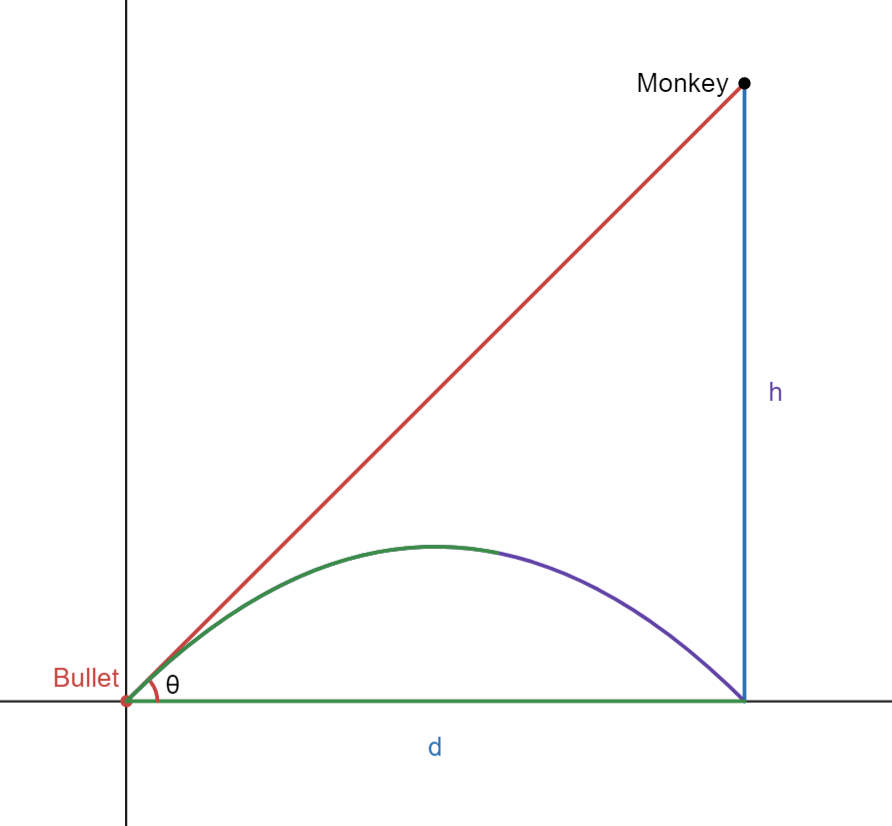
\includegraphics[width=0.5\linewidth]{Pictures/PS00/monkey_v2.png}
    \caption{Trajectory of Bullet}
    \label{fig:01-2b}
\end{figure}
\begin{itemize}
    \item \textbf{Way 1:} Impose a condition related to elapsed time (I’m being deliberately vague here because I want you to think on your own what that condition needs to be, in words).
    
    Suppose the Monkey is at height $h$. We have the following equation
    \[
    h = \frac{1}{2}gt^2
    \]
    The time it takes the monkey to fall to the ground is given by
    \[
    t_{max} = \sqrt{\frac{2h}{g}}
    \]
    This means that the bullet have to reach the monkey before $t_{max}$, or before the monkey hits the ground. If the parabolic trajectory the bullet travels takes exactly $t_{max}$ to reach the monkey at the same time it hits the ground. We can define the vertical component of the bullet by
    \[
    v_{b,\perp} = v_b\sin\theta_0
    \]
    The time it take the bullet to complete a up-and-down motion can be written as
    \[
    \frac{t_{max}}{2} = \frac{v_b\sin\theta_0}{g}
    \]
    Substitute our expression for $t_{max}$ to this equation, we can find the speed of the bullet needed to meed this minimum criteria.
    \[
    v_b = \frac{\sqrt{2hg}}{2\sin\theta_0} = \frac{1}{\sin\theta_0}\sqrt{\frac{hg}{2}}
    \]

    
    \item \textbf{Way 2:} Impose a condition related to horizontal displacement of the projectile (again, I’m being vague for the same reason).

    Here, we define the horizontal distance between the monkey and the muzzle to be $d_{b,m}$. The bullet has to travel a parabolic curve whose intersection with the ground, or the 2 roots, has to be the muzzle and the position where the monkey falls down. We can find the relationship between $h$ and $d$ defined by 
    \[
    \tan\theta_0 = \frac{h}{d}
    \]
    since the gunner is directly aiming at the monkey. We see that the bullet have to travel the horizontal displacement $d$ while finishing a complete up-and-down motion, and they should complete these motion at the same time. Therefore, we can set up the following equality
    \[
    \frac{d}{v_b\cos\theta_0} = \frac{2v_b\sin\theta_0}{g}
    \]
    cross multiply, we have
    \[
   2 v_b^2\sin\theta_0\cos\theta_0 = dg
    \]
    Note that $\tan\theta_0 = \frac{h}{d}$, we have $d = \frac{h}{\tan\theta_0}$. Substitute
    \[
    2 v_b^2\sin\theta_0\cos\theta_0 = \frac{hg}{\tan\theta_0}
    \]
    We know that $\tan\theta = \frac{\sin\theta}{\cos\theta}$, we can keep doing substitution
    \[
    2 v_b^2\sin\theta_0\cos\theta_0  = \frac{hg\cos\theta_0}{\sin\theta_0}
    \]
    We can cancel the $\cos\theta_0$ term, and simplify
    \[
    v_b = \sqrt{\frac{hg}{2\sin^2\theta_0}} = \frac{1}{\sin\theta_0}\sqrt{\frac{hg}{2}}
    \]
    This is the same result obtained from the first way. 

    
\end{itemize}

\textbf{(c)} For a different perspective on how to arrive at a correct answer to (a), let’s analyze the situation in a frame whose axes are oriented parallel to the ground’s axes but whose origin is attached to the monkey. In this frame (i.e. relative to the monkey), determine:

\begin{enumerate}[i.]
    \item the acceleration of the projectile,

    The bullet is not accelerating with respect to the monkey.
    \[
    \mathbf{a} = \mathbf{o}
    \]
    \item its initial velocity,

    The initial velocity is the same as it would be observed by the gunner, $\mathbf{v}_0$
    \[
    \mathbf{v_0} = v_b\cos\theta_0 \unx + v_b\sin\theta_0 \uny
    \]
    \item its initial position,

    The initial position is $\mathbf{r}_0$
    \[
    \mathbf{r_0} = -d\unx -h\uny
    \]
    \item its velocity as a function of time

    The velocity is constant through time.
    \[
    \mathbf{v}(t) = \mathbf{v}_0
    \]
    \item its position as a function of time.

    The position as a function of time is linear. And it is 
    \[
    \mathbf{r}(t) = \mathbf{r}_0 + \mathbf{v}_0t
    \]


(\textbf{NOTE} that the answers to (i)–(v) are vectors). Finally:


    \item Demonstrate that the projectile will hit the monkey and compute how long after launch the impact takes place (provided, of course, that we had \(v_0 > v_0, \text{min}\)).
    Since the relationship is linear and the position vector is co-linear with the velocity vector, we can express time as
    \[
    t = \frac{\abso{\mathbf{r}_0}}{\abso{\mathbf{v}_0}}
    \]

    
\end{enumerate}


\section{1 circle, 3 frames}

\textbf{(a)} In an inertial frame \(S\) with a standard orthonormal Cartesian \(\hat{x}, \hat{y}, \hat{z}\) basis, a particle moves clockwise at constant speed \(v\) in a circle of radius \(R\) in the \(x\)-\(y\) plane, centered at \((x = 0, y = 0, z = 0)\). At \(t = 0\), the particle is at \((x = R, y = 0, z = 0)\).

\begin{enumerate}
    \item[(i)] In terms of \(v\) and \(R\), what is the angular speed \(\omega\) of the particle in rad/unit time? Go ahead and use \(\omega\) in all your subsequent answers (it’ll reduce how much you have to write and make expressions look less busy).

    \[
    v = r\omega
    \]

    
    \item[(ii)] Write down the position, velocity, and acceleration of this particle as functions of time (these are \textbf{vectors}—express your answers using the Cartesian basis listed above).

    \[
    \begin{cases}
        \mathbf{r} = R\cos(\omega t) \unx - R\sin(\omega t)\uny\\
        \mathbf{v} = -R\omega\sin(\omega t)\unx  - R\omega\cos(\omega t)\uny\\
        \mathbf{a} = -R\omega^2\cos(\omega t) \unx + R\omega^2\sin(\omega t)\uny
    \end{cases}
    \]


    
\end{enumerate}

\textbf{(b)} Now imagine a frame \(S'\) with axes and basis vectors parallel to the corresponding ones in \(S\) and that moves at constant speed \(v\) in the \(-\hat{x}\) direction along the line \(y = -R\) as viewed in frame \(S\), i.e., the speed of \(S'\) as viewed by \(S\) is the same as the translational speed of the circulating particle as viewed by \(S\).

\begin{enumerate}
    \item[(i)] Write down the position, velocity, and acceleration of the same particle as functions of time as viewed in \(S'\). Since the axes of \(S'\) are aligned with those of \(S\), feel free to share the \(\hat{x}, \hat{y}, \hat{z}\) basis vectors between them.

    \[
    \begin{cases}
        \mathbf{r'}(t) = \paren{R\cos\paren{\omega t} + vt}\unx + \paren{-R\sin\paren{\omega t} + R}\uny\\
        \mathbf{v'}(t) = \paren{-R\omega\sin\paren{\omega t}+ v}\unx  -R\omega\cos\paren{\omega t}\uny\\
        \mathbf{a'}(t)  = -R\omega^2\cos(\omega t) \unx + R\omega^2\sin(\omega t)\uny
    \end{cases}
    \]

    
    
    \item[(ii)] In frame \(S'\), what does the trajectory traced out by the particle look like?

    It will look like a cycloid that curves down, concave down. 



    \item[(iii)] In frame \(S'\), what’s going on with the velocity of the particle at the lowest points (where the trajectory has cusps)?

    At the cusps of the motion, the velocity of the particle is 0. Since the velocity vector will be pointing at the opposite direction to where the frame $S'$ is moving, therefore they sort of cancels. Since the rotation starts at $x=R$ for $S$, it should reach the cusps at $\omega t= \frac{\pi}{2} 2\pi k$ for some $k \in \Z$. And if we throw this info in, we have $\mathbf{v}_{cusps} = -v \unx$, which when working together with the velocity of $S$ moving relative to $S'$, or $v_S = v\unx$, it becomes 0. 
\end{enumerate}

Go watch the following \textbf{black \& white video} from the 1960s about frames-of-reference (watch the whole thing — it’s worth it). There’s a scene around minute 9:00 where Prof. Hume demonstrates precisely this situation. A small ball is moving in a vertical circle at constant speed (because it’s attached to a spinning disc), and then he lets the whole disc move horizontally on a track at constant speed relative to the ground. A Sharpie-type marker on the ball traces out a curve on a piece of plexiglass (that’s stationary relative to the ground) as it coasts by. See the shape drawn out by the marker? You just determined a parametric equation for that shape. The expressions for \( x(t), y(t) \) you just derived trace out a \textbf{cycloid}. There is a nice description and animation on \href{https://en.wikipedia.org/wiki/Cycloid}{this Wikipedia page}.

But appreciate what you’ve just done. Generating the equation of the cycloid starting from frame \(S'\) isn’t easy. But once you realize that, in a frame that co-moves with the center of the rolling disc, the cycloid is just a particle moving in a circle at constant speed, then life becomes easier. All you need to know is (1) how to write down an equation for the trajectory in that co-moving frame (and circles are fairly easy, so we do know how to do this), and (2) how to \textit{translate} your description in this co-moving frame back into the “ground” frame.

\textbf{This is an extremely powerful and recurring theme in the way physics tries to analyze the world!} Don’t default to analyzing everything from scratch. Instead, look for the familiar in the unfamiliar, and avail yourself of tools like frame-shifting to help make things look familiar.

\textbf{(c)} Let’s see what the circle would look like from yet a third point of view. Now imagine a frame \(S''\) (again with standard axes and basis vectors aligned with those of \(S\)) whose origin, as viewed from frame \(S\), moves along the \(z\)-axis of \(S\) in the \(-\unz\) direction at \(v\) (same speed that \(S\) says the circulating particle has). Same drill:

\begin{enumerate}
    \item[(i)] Write down the position, velocity, and acceleration of the same particle as functions of time as viewed in \(S''\).

    \[
    \begin{cases}
        \mathbf{r''}(t)  = R\cos(\omega t) \unx - R\sin(\omega t)\uny + vt\unz \\
        \mathbf{v''}(t)  = -R\omega\sin(\omega t)\unx  - R\omega\cos(\omega t)\uny + v\unz\\
        \mathbf{a''}(t)  = -R\omega^2\cos(\omega t) \unx + R\omega^2\sin(\omega t)\uny
    \end{cases}
    \]

    \item[(ii)] In frame \(S''\), what does the trajectory traced out by the particle look like? What is this shape called? (Yet again, you have used physics to answer a geometry problem.)

    This thing will trace out a helix in the $+\unz$ axis. 

    
    \item[(iii)] In this frame, how does the speed of the particle vary in time?

    There is an extra segment of $v\unz$ that directs the velocity vector in the $\unz$ direction away from the $xy$ plane. 
    
    \item[(iv)] In this frame, what is the ratio of the magnitude of the acceleration to the magnitude of the velocity?

    Let us use $\varphi$ to define the ratio.
    \[
    \varphi = \frac{R\omega^2}{\sqrt{R^2\omega^2+v^2}}
    \]
    Since $v = R\omega$, we can keep simplifying the expression
    \[
    \varphi = \frac{\omega}{\sqrt{2}}
    \]

    
\end{enumerate}


\section{Some non-circles}

\begin{enumerate}
    \item[T1 1.11] \( \mathbf{r}(t) = b\cos(\omega t)\unx + c\sin(\omega t)\uny \)

    This is an eclipse.
    
    \item[T1 1.12]\( \mathbf{r}(t) = b\cos(\omega t)\unx + c\sin(\omega t)\uny + v_0t\unz \)

    This is an elliptical helix. 
\end{enumerate}



\section{1 puck, 3 frames}

\textbf{1.26**} The hallmark of an inertial reference frame is that any object which is subject to zero net force will travel in a straight line at constant speed. To illustrate this, consider the following: I am standing on a level floor at the origin of an inertial frame \(S\) and kick a frictionless puck due north across the floor.

\textbf{(a)} Write down the \(x\) and \(y\) coordinates of the puck as functions of time as seen from my inertial frame. (Use \(x\) and \(y\) axes pointing east and north respectively.) Now consider two more observers, the first at rest in a frame \(S'\) that travels with constant velocity \(v\) due east relative to \(S\), the second at rest in a frame \(S''\) that travels with constant \textit{acceleration} due east relative to \(S\). (All three frames coincide at the moment when I kick the puck, and \(S''\) is at rest relative to \(S\) at that same moment.)

The coordinate as seen in the frame of $S$ will be 
\[
r_S = (0,v_N t)
\]
Where $v_N$ is the speed where the puck is going to the North.




\textbf{(b)} Find the coordinates \(x', y'\) of the puck and describe the puck’s path as seen from \(S'\).

\[
r_{S'} = (-v_E t,v_N t)
\]

The path of the puck is seen as a straight line moving in the Northwest direction. 

\textbf{(c)} Do the same for \(S''\). Which of the frames is inertial?

The $x$ coordinate will move to the West since $S'$ is moving to the East. And for $S''$
\[
r_{S''} = \paren{-v_Et - \frac{1}{2}at^2, v_N t}
\]


The path for $S''$ will be curved, initially moving to Northwest and slowly leaning more and more towards West direciton. And $S''$ is not inertial since it is accelerating with respect to $S$ and $S'$ that are inertial.



\section{1 puck, 1 turntable, 2 frames}
\begin{enumerate}
    \item[T1 1.27]

    The ball in the rotating table perspective will move in from the edge of the table and go in a curved path and leave on the edge, leaving something like a bite off the apple logo.

    \item[T1 1.46] Consider the experiment of Problem 1.27, in which a frictionless puck is slid straight across a rotating turntable through the center \(O\).

\textbf{(a)} Write down the polar coordinates \(r, \phi\) of the puck as functions of time, as measured in the inertial frame \(S\) of an observer on the ground. (Assume that the puck was launched along the axis \(\phi = 0\) at \(t = 0\).)

Since we are initially on the line $\phi = 0$, or basically the $x$ axis, and the puck goes in a straight line in $S$ perspective, it's polar coordinate can be simply written as
\[
P_{S} = (R-v t, 0)
\]
Where $v$ is the speed of the puck, and it is moving along the $\phi = 0$ axis with the radius changing by a rate of $-vt$.

\textbf{(b)} Now write down the polar coordinates \(r', \phi'\) of the puck as measured by an observer (frame \(S'\)) at rest on the turntable. (Choose these coordinates so that \(\phi\) and \(\phi'\) coincide at \(t = 0\).) Describe and sketch the path seen by this second observer. Is the frame \(S'\) inertial?

\[
P_{S'} = \paren{ R - vt, -\omega t}
\]
Where $v$ is the speed of the puck, and the angle is changing at the rate which the round table is rotating. Since the round table is rotating clockwise, it is a $-\omega t$ rate. 

\end{enumerate}

\section{Is this frame inertial}
You’re getting a video feed on your phone from a camera inside a railway boxcar that has no windows. You have no idea where this boxcar is or how the camera is oriented inside it, but you know that the camera is affixed to a wall of the car, i.e. it’s not moving relative to the car’s interior. On your video screen, you see the following. The floor and ceiling look horizontal to you, i.e. you don’t need to tilt your phone to some weird angle to have the floor in the image be parallel to the floor you’re physically standing on. Hanging from the ceiling is a mass on a thin taut rope, only it’s not hanging perpendicular to the boxcar floor in the video. Instead, it’s hanging kind of down and left, making some noticeable angle with the ground, but the mass is otherwise stationary with respect to the boxcar interior. Assume that a frame attached to the ground on which you are physically standing while watching this video stream is inertial. Do you have enough evidence to determine whether the boxcar frame is inertial? If the answer is “yes”, then is that frame inertial or not? If the answer is “no”, then explain why you don’t have enough evidence.

We do not have enough evidence to show this frame is inertial or not. If the ball is \textit{hanging} on a rope, then the rope is under tension. Since there are tension force from the wire hanging the ball and it is not in a completely force free environment. Therefore we do not have enough evidence, that is, force-less environment. If we have information on whether the rope is under tension or not, we can draw a more definitive answer since it is the only thing contacting the ball. 


\section{1 block, 1 wedge, no friction anywhere}

This is the problem we started in class. A block of mass $m$ is initially at rest on a wedge of mass $M$ (also at rest) that makes an angle $\theta$ with the ground. There is no friction either between the block and the wedge or between the wedge and the floor. The system is released from rest. Determine:
\begin{figure}[!h]
    \centering
    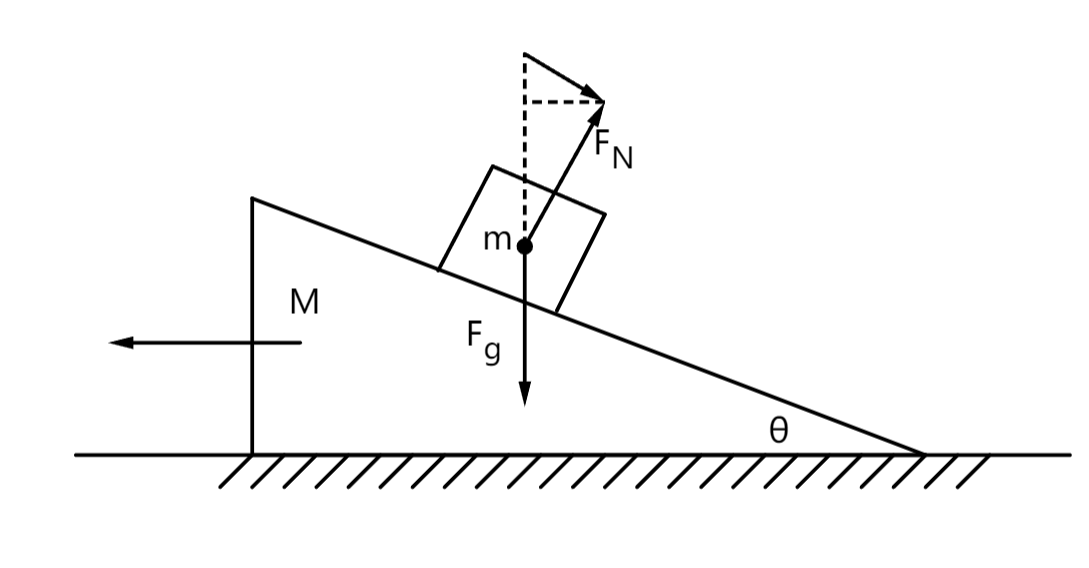
\includegraphics[width=0.5\linewidth]{Pictures/PS00/wedgeBlock.png}
    \caption{Moving Wedge and a Block}
    \label{fig:01-7}
\end{figure}

\begin{enumerate}
    \item the magnitudes of the accelerations of the block relative to the floor and of the wedge relative to the floor;

\textcolor{blue}{The lesson learned in this question is not to assert my previous knowledge of inertial frame without further consideration of acceleration. Newton's second law only works in inertial frames and we would have to conjure some extra information to make our system satisfy this criteria. And making some tweaks to our frame of reference so that the calculation is the easiest is also very important. In this question, we rotated the frame of reference to align with the \textit{net gravity} that we made up, so the problem would behave just as an introductory mechanics problem, except the algebra is more hell-ish. My previous answer was completely erroneous so I gray-ed out all of it.}

\textcolor{gray}{When the block is sliding down the wedge, it experiences the normal force $F_{N,w}$ from the wedge, and $F_g$ by gravity. We know that $F_g$ is given by
    \[
    F_{b,g} = mg
    \]
    And we can derive that the normal force is given by
    \[
    F_{N,w} = mg\cos\theta
    \]
    And a component that is parallel to the surface of the wedge on the block
    \[
    F_{bx,w} = mg\sin\theta
    \]
    We can use this force to find the acceleration of the block using Newton's second law in the wedge perspective, and is parallel to the surface of the wedge. This is also the case with respect to the floor. 
    \[
    a_{b,w} = a_{b,f} = g\sin\theta
    \]
    We can then use this to find the horizontal component, or $x$ component of this acceleration by
    \[
    a_{bx,w}=g\sin\theta\cos\theta
    \]
    Or simplified as
    \[
    a_{bx,w} = \frac{g}{2}\sin\paren{2\theta}
    \]
    We can find the force that is pushing the block in the $x$ direction using Newton's second law again
    \[
    F_{wx,b} = m\paren{a_{bx,w}} = mg\sin\theta\cos\theta
    \]
    We also know that the block exert a reaction in the opposite direction that drives the wedge in the $-x$ direction. We can find the following equality
    \[
    Ma_w = F_{wx,b} = mg\sin\theta\cos\theta
    \]
    Therefore the acceleration of the wedge relative to the ground can be found as
    \[
    a_{w,f} = \frac{mg}{M}\sin\theta\cos\theta
    \]
    Or simplified as
    \[
    a_{w,f} = \frac{mg\sin\paren{2\theta}}{2M}
    \]
    \item the magnitude of the contact force that the wedge applies to the block. The magnitude of the contact force is the magnitude of the normal force the wedge applies to the wedge, given by 
    \[
    F_{N,w} = mg\cos\theta
    \]}

Mistakes in original answer is gray-ed out.


\begin{large}
    \textbf{Correction}
\end{large}


\textcolor{blue}{The problem is solved correctly when we do not treat the wedge as an inertial frame without additional tweaks. Here, since the block is accelerating in the opposite direction, we introduce a fictional gravity $A = -a_{M,f}$ that compensates for the acceleration of the wedge.}

\textcolor{blue}{Now, we can define a total gravity that is the result of the real gravity and the fake gravity. as $g'$. And the angle $g'$ makes with the real gravity is defined as $\phi$. Now, we define a new frame of reference that is tilted $\phi$ degrees such that $g'$ points straight in the $-\uny$ direction. And in this frame, we can treat the wedge frame as somewhat inertial. And the acceleration down the wedge, or parallel to the wedge in the wedge perspective is
\[
a_{b,w} = a_b' = g'\sin\paren{\theta+\phi}
\]
We denote it with $a_b'$}

\textcolor{blue}{We can use trig identities to expand and get
\[
a_b' = g'\sin\phi\cos\theta + g'\cos\phi\sin\theta
\]
We notice that $g = g'\cos\theta$ and the fake gravity $A = g'\sin\phi$, the whole thing simplifies to
\[
a_b' = A\cos\theta + g\sin\theta \tag{Eq.1}
\]
We can also use $g'$ to find the normal force, defined as
\[
F_N = mg'\cos\paren{\theta+\phi}
\]
We can use the trig identities again to expand this into
\[
F_N = mg'\cos\theta\cos\phi - mg'\sin\theta\sin\phi
\]
We can use the relationship just like before to arrive at
\[
F_N = mg\cos\theta - mA\sin\theta \tag{Eq.2}
\]
And we know that the normal force has a component of the acceleration of the wedge relative to the floor.
\[
F_N\sin\theta = MA 
\]
Throw in the normal force, we have
\[
mg\cos\theta\sin\theta - mA\sin^2\theta - MA = 0
\]
This simplifies to
\[
A = \frac{mg\cos\theta\sin\theta}{M+m\sin^2\theta} \tag{Eq.3}
\]
We also know that in the frame of the floor, we will call it $a_b$, the acceleration of the block is actually
\[
\textbf{a}_b = \textbf{a}'_b - A\unx \tag{Eq.4}
\]
And this is the last piece of the puzzle. We have to find $a_b'$ using Equation 1.
\[
a_b' = g\sin\theta\paren{\frac{M+m}{M+m\sin^2\theta}}
\]
And now we can work out the expression for the acceleration $a_b$, and that is
\[
\mathbf{a}_b = a'_b\paren{\cos\theta \unx -\sin\theta\uny} - A\unx
\]
And we can find the magnitude of the acceleration $a_b$ by
\[
a_b^2 = \paren{a'_b\cos\theta - A}^2 + \paren{a'_b\sin\theta}^2
\]
Now we can carry out this algebraically and substitute the expressions in, after simplification, we will find that
\[
a_b =\frac{g\sin\theta}{M+m\sin^2\theta} \sqrt{M^2+\sin^2\theta\paren{2M+m^2}}
\]
And the magnitude of the contact force is the magnitude of the normal force. With our previously established formula, we obtain that the normal force is
\[
F_N = mg\cos\theta - mA\sin\theta \quad A = \frac{mg\cos\theta\sin\theta}{M+m\sin^2\theta} 
\]}

        
\end{enumerate}
Express your answers only in terms of $m$, $M$, $\theta$, and constants of nature.




\section{1 Train, 1 Person, 1 Ball, 2 Frames}

\textbf{Problem 2-41.} A train moves along the tracks at a constant speed \(u\). A woman on the train throws a ball of mass \(m\) straight ahead with a speed \(v\) relative to herself.

\textbf{(a)} What is the kinetic energy gain of the ball as measured by a person on the train?

From the perspective of a person on the train, the kinetic energy gained by the ball is:
\[
\Delta E_{\text{K,t}} = \frac{1}{2}mv^2
\]
where \( \Delta E_{\text{K,t}} \) is the change in kinetic energy in the reference frame of the person on the train. This is also the work done by the woman, as no external forces act on the train in this frame.

\textbf{(b)} What is the kinetic energy gain of the ball as measured by a person standing by the railroad track?

In the ground frame, the ball’s velocity is the combination of the train's velocity \(u\) and the velocity \(v\) with which the woman throws the ball. Thus, the kinetic energy of the ball, as seen from the ground, is:
\[
E_{\text{ball,g}} = \frac{1}{2}m(u + v)^2 = \frac{1}{2}m(u^2 + 2uv + v^2)
\]
The initial kinetic energy of the ball (before it was thrown), as seen from the ground, was:
\[
E_{\text{ball,g,in}} = \frac{1}{2}mu^2
\]
The change in the kinetic energy, or the kinetic energy gained, as observed from the ground, is:
\[
\Delta E_{\text{K,g}} = E_{\text{ball,g}} - E_{\text{ball,g,in}} = \frac{1}{2}m(u^2 + 2uv + v^2) - \frac{1}{2}mu^2
\]
Simplifying:
\[
\Delta E_{\text{K,g}} = \frac{1}{2}m(2uv + v^2)
\]
where \( \Delta E_{\text{K,g}} \) is the energy gain in the ground frame.

\textbf{(c)} How much work is done by the woman throwing the ball?

In both the train frame and the ground frame, the work done by the woman is the same. The woman exerts force only on the ball, and since the train is not accelerating, her work is independent of the train’s motion. The work done by the woman, which is equal to the kinetic energy change of the ball in her frame, is:
\[
W_{\text{woman}} = \Delta E_{\text{K,t}} = \frac{1}{2}mv^2
\]
This work is the same in both the train frame and the ground frame because the train is moving at a constant speed.

\textbf{(d)} What is the work done by the train?

To calculate the work done by the train, we look at the difference between the total kinetic energy change observed from the ground and the work done by the woman. The change in energy observed from the ground is:
\[
\Delta E_{\text{K,g}} = \frac{1}{2}m(2uv + v^2)
\]
The work done by the woman is:
\[
W_{\text{woman}} = \frac{1}{2}mv^2
\]
Thus, the work done by the train is the difference between the energy change observed from the ground and the work done by the woman:
\[
W_{\text{train}} = \Delta E_{\text{K,g}} - W_{\text{woman}} = \frac{1}{2}m(2uv + v^2) - \frac{1}{2}mv^2
\]
Simplifying:
\[
W_{\text{train}} = muv
\]




\end{document}